\chapter{Implementación}\label{cap:implementacion}

\section{Introducción}
Este capítulo describe la implementación real del proyecto a nivel de repositorio,
notebooks y artefactos de datos. El objetivo es mostrar cómo el diseño del
capítulo anterior se materializa en entregables ejecutables y verificables.

\section{Herramientas y versiones}
Las herramientas principales utilizadas son:
\begin{itemize}
	\item \textbf{Apache Spark 3.5.1} para procesamiento distribuido.
	\item \textbf{Apache Zeppelin 0.11.1} para notebooks y visualización integrada.
	\item \textbf{Python 3 + PySpark} para enriquecimiento geográfico y mapas.
	\item \textbf{Folium} para generación de mapas coropléticos interactivos.
	\item \textbf{Docker Compose} para levantar servicios en local.
	\item \textbf{Git/GitHub} para control de versiones y trazabilidad.
\end{itemize}

Dependencias Python adicionales instaladas en el contenedor:
\begin{itemize}
	\item \texttt{geopandas}, \texttt{pyogrio} (para convertir shapefile a GeoJSON)
	\item \texttt{folium} (para mapas coropléticos)
	\item \texttt{numpy<2}, \texttt{pyarrow} (compatibilidad de datos)
\end{itemize}

\section{Estructura implementada}
El repositorio final se organiza de la siguiente forma:
\begin{itemize}
	\item \texttt{data/}: Parquet de entrada, shapefile, GeoJSON generado,
	script auxiliar \texttt{convert.py} y los 14 CSVs de indicadores exportados.
	\item \texttt{notebooks/}: los dos notebooks de Zeppelin (análisis principal
	y mapas) más una versión del notebook de mapas ya ejecutada.
	\item \texttt{docs/}: memoria LaTeX y documentación del proyecto.
	\item \texttt{logs/}: directorio de logs de Zeppelin.
\end{itemize}

\section{Orquestación con Docker Compose}
La ejecución local utiliza tres servicios:
\begin{itemize}
	\item \texttt{zeppelin}: interfaz notebook en el puerto \texttt{8080}.
	\item \texttt{spark-master}: coordinador Spark en \texttt{7077},
	con interfaz web en \texttt{8081}.
	\item \texttt{spark-worker-1}: nodo de cómputo con 3 GB de memoria
	y 2 núcleos.
\end{itemize}

Los volúmenes Docker montan \texttt{./data} como \texttt{/data} dentro de los
contenedores, de forma que tanto Spark como Python acceden al mismo directorio
de datos. Esta topología mantiene coherencia con un esquema distribuido real,
pero con complejidad controlada para entorno académico.

\section{Script auxiliar: generación de GeoJSON}
El único script fuera de los notebooks es \texttt{data/convert.py}, que convierte
el shapefile de zonas TLC a GeoJSON:

\begin{lstlisting}[language=python,caption={Script de conversión shapefile a GeoJSON}]
import geopandas as gpd
import pandas as pd

gdf = gpd.read_file('/data/taxi_zones.shp')
gdf = gdf.to_crs(epsg=4326)
gdf.to_file('/data/nyc_taxi_zones.geojson', driver='GeoJSON')
\end{lstlisting}

Se ejecuta una única vez dentro del contenedor Zeppelin:
\begin{lstlisting}[language=bash,caption={Ejecución del script de conversión}]
docker exec -u root -it zeppelin bash -c \
  "/opt/conda/envs/python_3_with_R/bin/python3 /data/convert.py"
\end{lstlisting}

\section{Implementación de los notebooks de Zeppelin}
El entregable analítico principal consta de dos notebooks:
\begin{itemize}
	\item \texttt{Análisis Taxis Nueva York.zpln}: notebook principal con carga,
	limpieza, análisis y exportación de indicadores.
	\item \texttt{Análisis Taxis Nueva York Mapas.zpln}: notebook de visualización
	geográfica con mapas coropléticos Folium.
\end{itemize}

Adicionalmente, se incluye \texttt{Análisis Taxis Nueva York Mapas (Ejecutados).zpln},
una versión del notebook de mapas ya ejecutada que permite revisar los resultados
visuales sin necesidad de relanzar el código.

\subsection{Notebook principal: flujo de análisis}

\subsection{Fase 1: carga y validación}
Se carga \texttt{/data/yellow\_tripdata\_2025-01.parquet}, se imprime esquema,
se cuenta el volumen de registros y se inspecciona una muestra inicial.

\subsection{Fase 2: limpieza y enriquecimiento en Spark}
En el notebook se aplican filtros de dominio adicionales, incluyendo:

\begin{itemize}
	\item \texttt{PULocationID} y \texttt{DOLocationID} en rango válido (1..263);
	\item pasajeros mínimos mayores o iguales a 1;
	\item tarifas e importes positivos;
	\item año de recogida esperado (2025);
	\item \texttt{dropoff} posterior a \texttt{pickup}.
\end{itemize}

También se traduce codificación numérica a etiquetas legibles de negocio para
\texttt{vendor}, tipo de pago, tarifa y bandera \texttt{store\_and\_fwd}.

\subsection{Fase 3: enriquecimiento geográfico}
Se lee \texttt{/data/nyc\_taxi\_zones.geojson}, se explota el array de
\texttt{features} y se realizan joins para añadir atributos de zona de recogida y
destino. Tras el enriquecimiento, se registra la vista temporal
\texttt{dfFinal} para consultas SQL.

\subsection{Fase 4: consultas de análisis y resultados}
Sobre la vista \texttt{dfFinal} se ejecutan consultas que sintetizan el
comportamiento del mes de enero de 2025. Los resultados se organizan en siete
bloques temáticos que cubren temporalidad, geografía, economía y tipología de
viaje.

\subsubsection*{a) Patrón horario de actividad}
La distribución horaria de viajes revela un patrón coherente con los ciclos de
actividad urbana de una gran metrópolis. La Figura~\ref{fig:ny-trips-hour}
muestra una curva con forma de campana asimétrica:
\begin{itemize}
\item el mínimo absoluto se registra a las 04:00 con apenas 12{,}175 viajes,
correspondiente al periodo de menor actividad urbana;
\item la demanda crece de forma sostenida a partir de las 06:00, coincidiendo con
el inicio de la jornada laboral y los desplazamientos al trabajo;
\item el máximo se alcanza a las 17:00 con 205{,}245 viajes, momento que
coincide con la salida generalizada del trabajo;
\item a las 18:00 el volumen apenas desciende (204{,}191 viajes), lo que indica
una hora punta prolongada, típica de ciudades con alta densidad de servicios.
\end{itemize}

Este patrón tiene implicaciones directas: sugiere que la oferta de vehículos
debería concentrarse entre las 15:00 y las 19:00 para cubrir la máxima demanda,
mientras que en madrugada la sobreoferta podría generar ineficiencia operativa.

\begin{figure}[H]
\centering
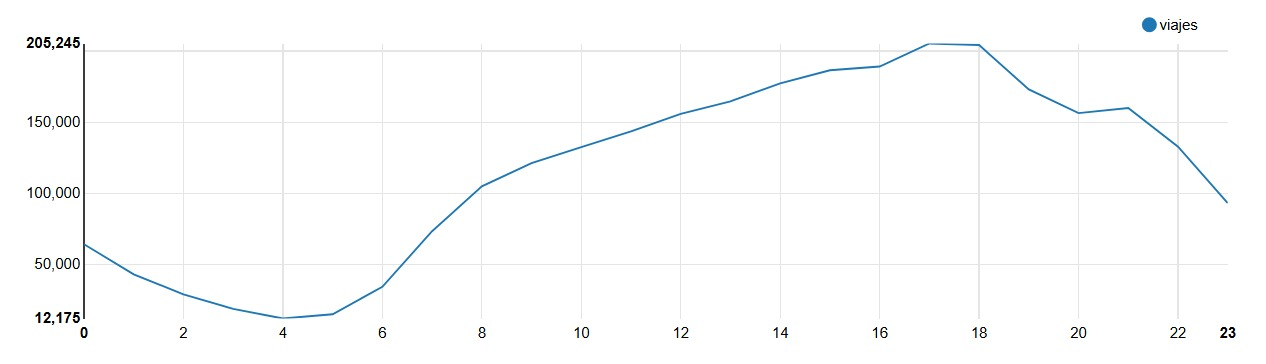
\includegraphics[width=0.95\textwidth]{figures/ny_trips_by_hour.jpeg}
\caption{Viajes por hora de recogida en enero de 2025. Se observa el mínimo
a las 04:00 (12{,}175) y el máximo a las 17:00 (205{,}245).}
\label{fig:ny-trips-hour}
\end{figure}

La Figura~\ref{fig:ny-fare-duration-hour} complementa el análisis anterior
al superponer tarifa media y duración media por hora. Se observa que:
\begin{itemize}
\item la tarifa media presenta un pico notable a las 05:00 (26.46 USD),
explicable porque los viajes de madrugada tienden a ser más largos (por ejemplo,
trayectos nocturnos desde zonas de ocio al aeropuerto o a periferia);
\item entre las 09:00 y las 13:00 aparece un segundo máximo de duración
(hasta 22.84 min a las 12:00), posiblemente asociado a congestión en hora
intermedia;
\item durante la franja de mayor demanda (17:00--18:00), la tarifa media se
estabiliza en torno a 18 USD con duraciones de unos 14 minutos, lo que refleja
viajes cortos pero frecuentes.
\end{itemize}

\begin{figure}[H]
\centering
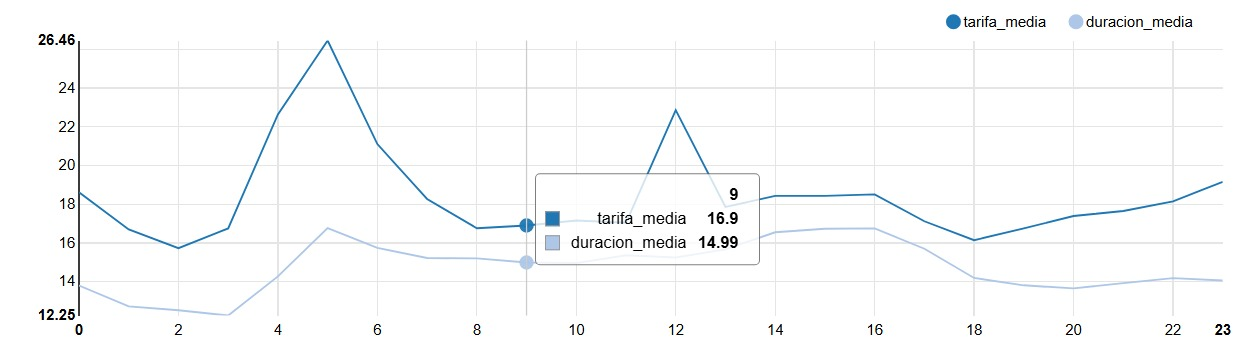
\includegraphics[width=0.95\textwidth]{figures/ny_fare_duration_by_hour.jpeg}
\caption{Tarifa media y duración media por hora de recogida. El pico de tarifa
a las 05:00 (26.46 USD) se explica por viajes largos nocturnos.}
\label{fig:ny-fare-duration-hour}
\end{figure}

\subsubsection*{b) 1 de enero frente al resto del mes}
El 1 de enero es el principal festivo del año y su comportamiento difiere
sustancialmente del patrón habitual. La Figura~\ref{fig:ny-jan1-vs-rest}
compara la media de viajes por hora del 1 de enero frente al promedio diario
del resto del mes:
\begin{itemize}
\item durante la madrugada (00:00--04:00), el 1 de enero supera ampliamente al
resto: a las 00:00 registra 5{,}543 viajes frente a los 1{,}977 habituales,
un incremento del 180\%, explicado por las celebraciones de Año Nuevo;
\item ambas series convergen sobre las 05:00, donde se alcanza el mínimo común
(343 viajes en día 1);
\item a partir de las 08:00, el resto de días domina con claridad, alcanzando
un máximo de 6{,}709 viajes por día a las 17:00, frente a los 4{,}246 del
festivo.
\end{itemize}

Este contraste evidencia que los eventos extraordinarios alteran drásticamente
la distribución de demanda y refuerza la importancia de segmentar el análisis
temporal para no distorsionar métricas agregadas.

\begin{figure}[H]
\centering
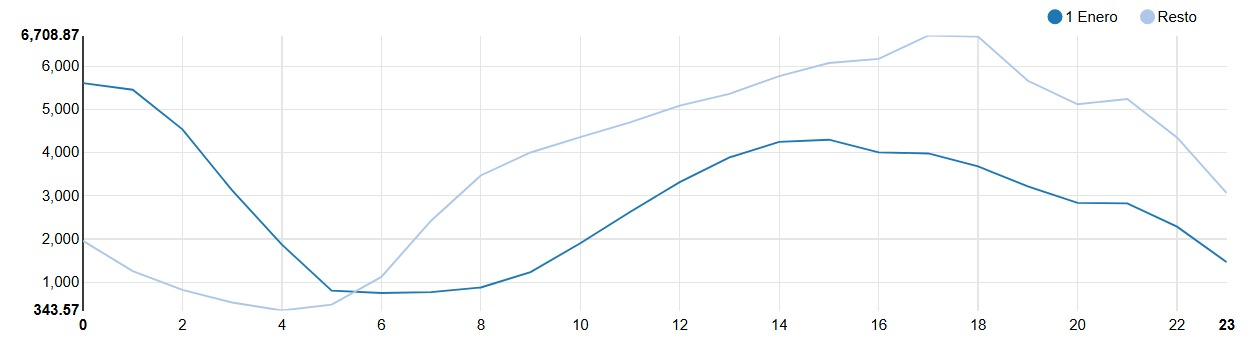
\includegraphics[width=0.98\textwidth]{figures/ny_jan1_vs_rest_by_hour.jpeg}
\caption{Media de viajes por hora: 1 de enero frente al promedio del resto
del mes. La madrugada del festivo muestra un comportamiento invertido respecto
al patrón diario normal.}
\label{fig:ny-jan1-vs-rest}
\end{figure}

\subsubsection*{c) Diferencias por distrito de recogida}
La Figura~\ref{fig:ny-borough-speed-cost} presenta indicadores operativos
agregados por distrito de recogida. Los contrastes son muy marcados:
\begin{itemize}
\item \textbf{Manhattan}: distancia media de solo 2.20 millas con velocidad
de 10.13 mph y un coste por milla de 6.50 USD. Los viajes cortos en zona
de alta congestión explican la baja velocidad y el elevado coste relativo.
\item \textbf{Queens}: 12.54 millas de media con 22.35 mph y 4.43 USD por
milla. Su proximidad a los aeropuertos JFK y LaGuardia genera viajes más
largos y rápidos.
\item \textbf{Bronx}: la mayor distancia media (17.03 millas) y la mayor
velocidad (22.28 mph), con el coste por milla más bajo (2.12 USD), lo que
refleja recorridos por vías rápidas con menor congestión.
\item \textbf{EWR} (Newark Airport): con 77.67 USD de tarifa media, casi
5 veces superior a Manhattan, pero a 31.37 mph, mostrando el perfil típico
de traslado interurbano al aeropuerto de Nueva Jersey.
\end{itemize}

Estos datos confirman que la movilidad en taxi no es homogénea: cada distrito
tiene un perfil operativo distinto que afecta directamente a ingresos,
eficiencia y experiencia del pasajero.

\begin{figure}[H]
\centering
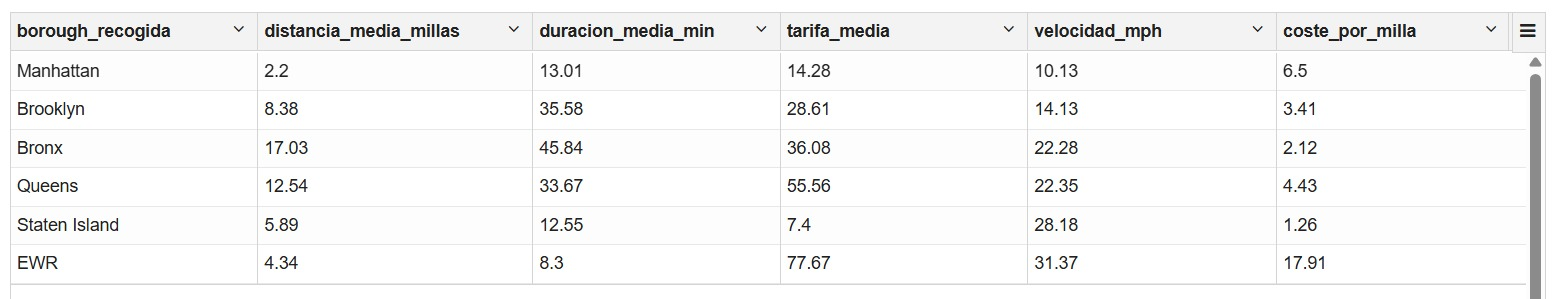
\includegraphics[width=0.95\textwidth]{figures/ny_borough_speed_cost.jpeg}
\caption{Indicadores operativos por distrito de recogida: distancia media,
duración, tarifa, velocidad y coste por milla.}
\label{fig:ny-borough-speed-cost}
\end{figure}

\subsubsection*{d) Viajes estándar vs aeropuerto}
La Figura~\ref{fig:ny-trip-type} compara los dos grandes segmentos de
servicio. Las diferencias son significativas en todos los indicadores:
\begin{itemize}
\item los viajes estándar dominan en volumen (2{,}696{,}555 frente a 94{,}614
de aeropuerto, ratio 28.5:1);
\item sin embargo, el viaje medio a aeropuerto recorre 17.71 millas frente a
2.65 (6.7 veces más), dura 44.66 minutos frente a 13.99 y genera una tarifa
media de 70.88 USD frente a 16.10;
\item la propina media de aeropuerto (11.91 USD) triplica la estándar
(3.18 USD), posiblemente porque el pasajero valora más un servicio puerta a
puerta con equipaje;
\item el porcentaje de propina es similar (16.8\% vs 19.7\%), lo que indica
que la diferencia en propina absoluta se debe a la mayor tarifa base, no a un
comportamiento más generoso.
\end{itemize}

\begin{figure}[H]
\centering
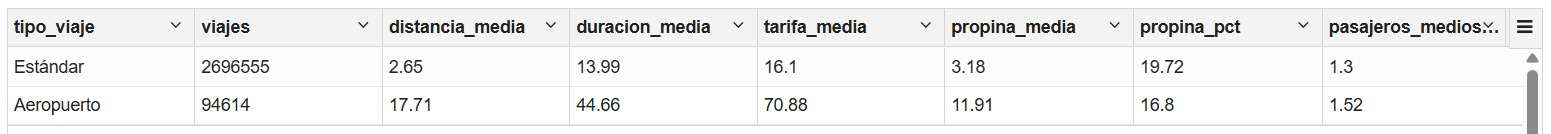
\includegraphics[width=0.92\textwidth]{figures/ny_trip_type_comparison.jpeg}
\caption{Comparativa entre viajes estándar y de aeropuerto: volumen, distancia,
duración, tarifa, propina y pasajeros medios.}
\label{fig:ny-trip-type}
\end{figure}

\subsubsection*{e) Franjas horarias y tipo de semana}
Para capturar la interacción entre momento del día y tipo de jornada, se
definieron cuatro franjas horarias: mañana (6--12h), tarde (12--18h), noche
(18--23h) y madrugada (23--6h). La Figura~\ref{fig:ny-timeslot-weektype}
muestra los resultados por viajes por día:
\begin{itemize}
\item la \textbf{tarde} es la franja dominante tanto en laborables
(35{,}066 viajes/día) como en fin de semana (33{,}678), con diferencia
mínima entre ambos;
\item la \textbf{mañana} presenta la mayor brecha: los laborables superan al
fin de semana en un 51\% (21{,}000 vs 14{,}000 viajes/día), reflejando los
desplazamientos al trabajo;
\item la \textbf{noche} muestra también más actividad en laborables
(28{,}000 vs 23{,}000), posiblemente por vuelta a casa tras jornada laboral;
\item la \textbf{madrugada} es la única franja donde el fin de semana supera
a los laborables (14{,}000 vs 6{,}000), consecuencia directa del ocio nocturno.
\end{itemize}

\begin{figure}[H]
\centering
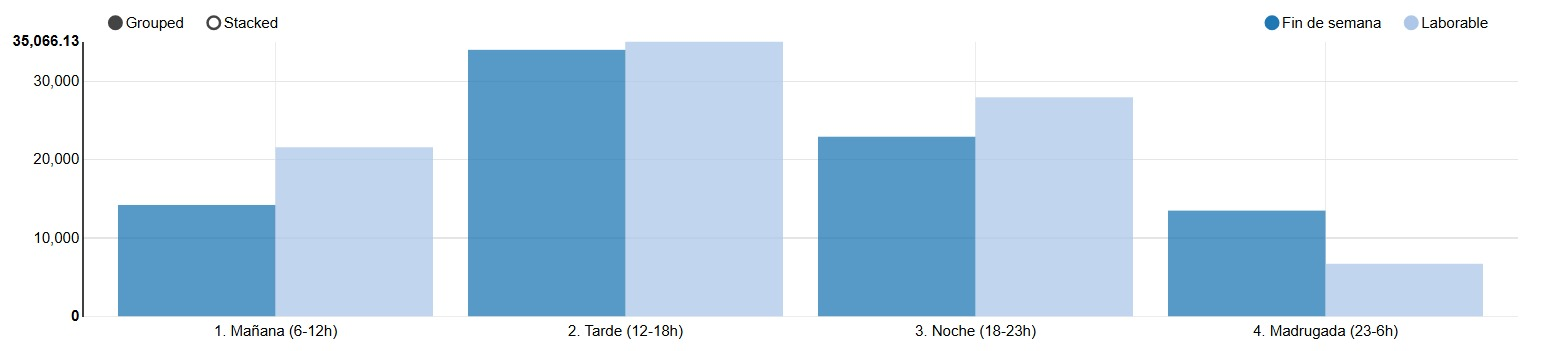
\includegraphics[width=0.95\textwidth]{figures/ny_timeslot_weektype.jpeg}
\caption{Viajes por día según franja horaria y tipo de semana. La madrugada es
la única franja donde el fin de semana supera a los laborables.}
\label{fig:ny-timeslot-weektype}
\end{figure}

\subsubsection*{f) Número de pasajeros}
La Figura~\ref{fig:ny-passengers} desglosa el servicio por ocupación del
vehículo. Los hallazgos son claros:
\begin{itemize}
\item los viajes de \textbf{1 pasajero} representan el 79\% del total
(2{,}231{,}648 registros), con tarifa media de 17.50 USD;
\item con \textbf{2 pasajeros} se registran 389{,}587 viajes (13.8\%),
y la tarifa media sube a 19.87 USD, lo que sugiere viajes ligeramente más
largos compartidos;
\item de 3 a 6 pasajeros el volumen desciende progresivamente (86{,}800,
53{,}995, 17{,}327 y 11{,}805 respectivamente), pero la tarifa media aumenta
hasta 21.38 USD para 4 pasajeros;
\item la propina media se mantiene estable entre 2.92 y 3.68 USD
independientemente de la ocupación, lo que indica que no se ajusta al número
de beneficiarios del servicio;
\item la distancia media es también estable (entre 2.92 y 3.68 millas),
lo que descarta que viajes con más pasajeros sean sistemáticamente más largos.
\end{itemize}

\begin{figure}[H]
\centering
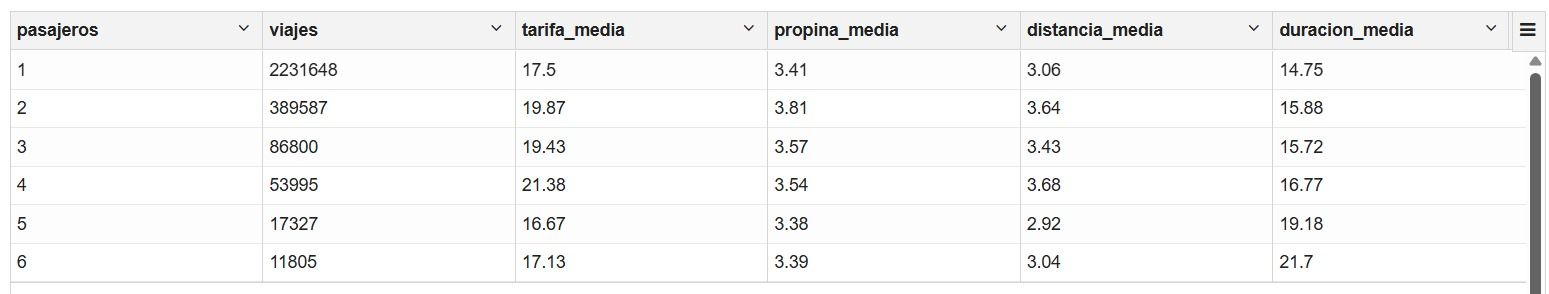
\includegraphics[width=0.95\textwidth]{figures/ny_passengers_trips_fare.jpeg}
\caption{Volumen de viajes, tarifa media, propina, distancia y duración
según número de pasajeros.}
\label{fig:ny-passengers}
\end{figure}

\subsubsection*{g) Balance recogidas-destinos por distrito}
La dinámica territorial se estudia mediante dos visualizaciones complementarias.
La Figura~\ref{fig:ny-pickup-vs-dest} muestra el porcentaje relativo de
recogidas frente a destinos por distrito, mientras que la
Figura~\ref{fig:ny-balance-borough} presenta la diferencia neta.

Los resultados revelan desequilibrios territoriales significativos:
\begin{itemize}
\item \textbf{Queens} es el mayor emisor neto con +119{,}591 viajes
(más recogidas que destinos), consistente con su función de acceso
aeroportuario: los taxis recogen pasajeros que aterrizan y los llevan a
Manhattan u otros distritos;
\item \textbf{Brooklyn} es el mayor receptor neto con -81{,}809 viajes,
indicando que recibe más viajes de los que genera, posiblemente por
desplazamientos residenciales de vuelta desde Manhattan;
\item \textbf{Manhattan} muestra un ligero déficit (-27{,}000 aprox.),
sorprendente dado su papel central, pero explicable porque el alto volumen
de recogidas y destinos casi se compensa;
\item \textbf{EWR} presenta un fuerte desequilibrio porcentual
(1.5\% de recogidas vs 98.99\% de destinos), lógico para un aeropuerto
donde predominan las llegadas en taxi;
\item \textbf{Staten Island} muestra un patrón similar con predominancia
clara de destinos (89\%) sobre recogidas (10\%).
\end{itemize}

\begin{figure}[H]
\centering
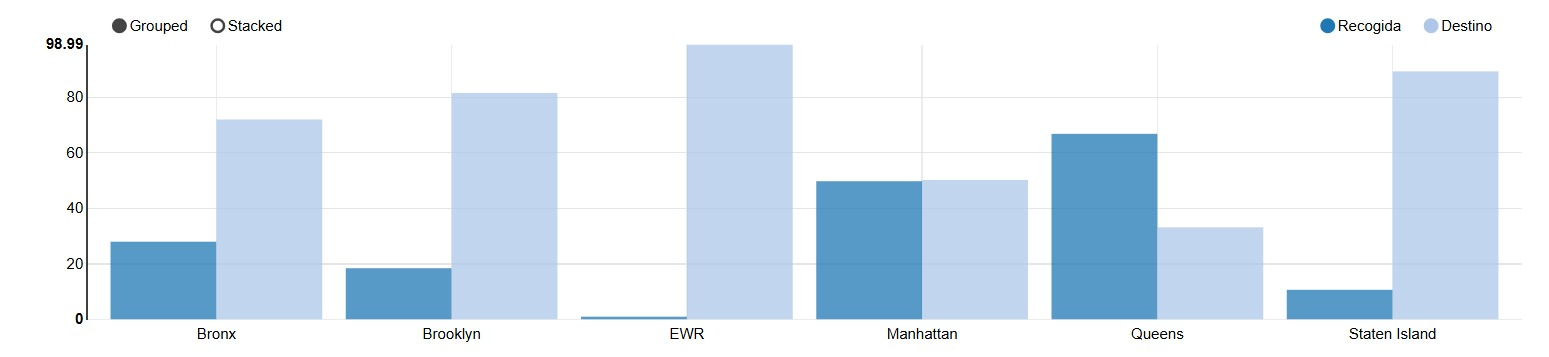
\includegraphics[width=0.95\textwidth]{figures/ny_pickup_vs_destination_by_borough.jpeg}
\caption{Proporción de recogidas frente a destinos por distrito. EWR y
Staten Island muestran los mayores desequilibrios relativos.}
\label{fig:ny-pickup-vs-dest}
\end{figure}

\begin{figure}[H]
\centering
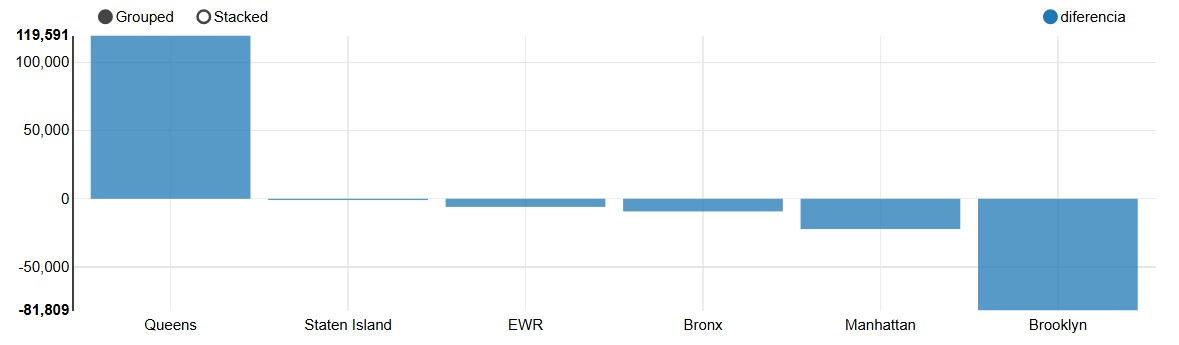
\includegraphics[width=0.95\textwidth]{figures/ny_pickup_destination_balance.jpeg}
\caption{Diferencia neta entre recogidas y destinos por distrito. Queens
como emisor neto (+119{,}591) y Brooklyn como receptor neto (-81{,}809).}
\label{fig:ny-balance-borough}
\end{figure}

\subsection{Fase 5: interpretación consolidada}
La secuencia de consultas y gráficas permite construir una lectura integrada del
servicio de taxi en Nueva York que articula cuatro dimensiones de análisis:

\begin{itemize}
	\item \textbf{Demanda temporal}: la actividad sigue ciclos predecibles
	(mínimo a las 04:00, máximo a las 17:00), con alteraciones claras en
	festivos y fines de semana.
	\item \textbf{Heterogeneidad espacial}: cada distrito tiene un perfil
	operativo propio en velocidad, distancia y coste, condicionado por
	infraestructura viaria y función urbana.
	\item \textbf{Segmentación de servicio}: los viajes a aeropuerto,
	aunque minoritarios en volumen, generan tarifas e ingresos por viaje
	muy superiores al servicio estándar.
	\item \textbf{Dinámica origen-destino}: los flujos no son simétricos;
	existen distritos emisores netos (Queens) y receptores netos
	(Brooklyn), lo que refleja patrones reales de movilidad residencial y
	funcional.
\end{itemize}

Adicionalmente, para cada zona TLC se exportaron indicadores detallados tanto
por origen como por destino:
\begin{itemize}
	\item \textbf{Origen (pickup)}: viajes, tarifa media, propina media,
	distancia media, duración media, viajes hora pico/valle e ingresos totales.
	\item \textbf{Destino (dropoff)}: mismos indicadores agregados por
	\texttt{DOLocationID}.
\end{itemize}

Esta separación permite comparar la dinámica de entrada y salida de cada zona
a nivel granular, más allá de la agregación por distrito.

\section{Artefactos de salida}
Tras ejecutar el flujo completo, los artefactos generados son:

\begin{itemize}
	\item \textbf{Datos de entrada}: \texttt{data/yellow\_tripdata\_2025-01.parquet}
	\item \textbf{GeoJSON generado}: \texttt{data/nyc\_taxi\_zones.geojson}
	\item \textbf{Indicadores por zona de origen} (7 CSVs):
	\texttt{viajes\_por\_zona.csv}, \texttt{tarifa\_por\_zona.csv},
	\texttt{propina\_por\_zona.csv}, \texttt{distancia\_por\_zona.csv},
	\texttt{duracion\_por\_zona.csv}, \texttt{ingresos\_por\_zona.csv},
	\texttt{viajes\_hora\_pico.csv}
	\item \textbf{Indicadores por zona de destino} (7 CSVs):
	\texttt{viajes\_por\_destino.csv}, \texttt{tarifa\_por\_destino.csv},
	\texttt{propina\_por\_destino.csv}, \texttt{distancia\_por\_destino.csv},
	\texttt{duracion\_por\_destino.csv}, \texttt{ingresos\_por\_destino.csv},
	\texttt{viajes\_hora\_valle.csv}
	\item \textbf{Mapas interactivos}: generados en HTML dentro del notebook
	de mapas con Folium.
\end{itemize}

\section{Conclusiones}
La implementación alcanzada cubre de extremo a extremo el caso de uso planteado:
ingesta de Parquet, calidad del dato, enriquecimiento geográfico, análisis
tabular, exportación de indicadores y visualización con mapas interactivos.
Los notebooks de Zeppelin no actúan como pruebas aisladas, sino como síntesis
operativa de todo el proyecto y base directa para defensa oral.